\chapter{Hydrogen Bond Dynamics of Water/Vapor Interfaces }\label{CHAPTER_HB}
There are two types of bonds in water: the stronger covalent bonds (molecular $\sigma$ bonds) within a single water molecule and 
the much weaker H-bonds between water molecules.
H-bonds play a critical role in the behaviour of bulk water,\cite{Eisenberg1969,Luzar1996,Cabane2005} water near interfaces,[] 
and aqueous solutions. \cite{Naslund2005} 
In this chapter, we will introduce the general concepts and methods of HB Dynamics (HBD)\cite{AL96,Luzar1996,DC87} used to analyze the structure 
and dynamic properties of bulk solutions and gas-liquid interfaces. 

\section{Definitions of Hydrogen Bond Population and Correlation Functions}
Luzar and Chandler [\cite{AL96}] have elucidated the HB dynamics of pure water, and
subsequently such analysis has been also extended to explore the HB dynamics
in complex situations, e.g., electrolytes, [\cite{AC00}] protein and  micellar surfaces. [\cite{SP05}]
There are temporal, geometric and energetic criteria to define HB. Here we use the geometric one.
Two water molecules are H-bonded only if their interoxygen distance between of specific tagged pair of water molecules 
is less than $r^{\text{c}}_{\text{OO}}=3.5$ \A \ and
the O-H$\cdots$O angle is less than $\phi^{\text{c}}=30^{\circ}$. [\cite{AKS86,JT90,SB02}] 
The value 3.5 \AA corresponds to the first-minimum position of the O--O RDF of water. [\cite{Sciortino1989}]   
The choice for the cutoff angle $\phi^{\text{c}}$ for water-water molecules is obtained by studying the average number of H-bonds,
as a function of $\phi^{\text{c}}$. \cite{Luzar1993} We call this definition of HB the ADH criterion. 
In order to compare the impact of different HB definitions on HB dynamics, we will also use another definition of HB in our analysis. 
When the distance between the oxygen atoms of two water molecules is less than 3.5 \AA, 
and the oxygen-hydrogen-oxygen included angle is greater than $120^{\circ}$, then we say that there is a HB between the two molecules. 
We denote this definition as the AHD definition of H bonds.
%The distance criteria of $R_{\text{OH}}$  was determined from the first minimum in the O--H RDF for SPC water. [\cite{HJCB81}]

% introduce h(t)
The configuration criterion above allows us to define a variable $h[r(t)] = h(t)$, HB population. 
The $h(t)$ has a value 1 when the particular tagged pair of molecules are bonded, and 0 otherwise. 
%=================
% added 2020-5-27: to show that h(t) is actually the fluctuation of itself (\delta h).
We know that the instantaneous fluctuation or deviation in a dynamical variable $A(t)$ from its time-independent equilibrium average $\langle A\rangle$ , 
is defined by [\cite{DC87}] 
$$
\delta A = A(t) - \langle A\rangle.
$$
For the $h(t)$, since the probability that a specific pair of molecules is bonded in a large system is extremely small, i.e., 
the time average of $h$ is zero, or  
$\langle h \rangle = 0$,
then
$$
\delta h(t) = h(t).
$$
Therefore, the $h(t)$ describe the instantaneous fluctuation $\delta h(t)$  of the HB population.  
%The behaviour of $r_{OO}(t)$  is depicted in Fig.\ref{fig:Ex30ps_hb}(a). We find that in the equilibrium system, $r_{OO}(t)$ looks chaotic.
%=================

While the equilibrium average of the $\delta h(t)$ is zero, but we can obtain useful information by considering the equilibrium 
correlations between fluctuations at different times. The correlation between the $\delta h(t)$ and the $\delta h(0)$ can be written as 
$$
\langle \delta h(0) \delta h(t)\rangle = \langle h(0)h(t)\rangle-\langle h \rangle^2 = \langle h(0)h(t)\rangle,
$$
where the averaging $\langle\cdots\rangle$ is to be performed over the ensemble of initial conditions $(r^N, p^N)$.


In this section, we will use three correlation functions to describe the HB dynamics of water/vapor interfaces of solutions,
the HB population correlation function \CHB, the survival probability \SHB and the reactive flux $k(t)$. [\cite{DCR83}]

\paragraph{Structure of HB Network}
One of the importrant characteristics of HB network is the average number of H-bonds per molecule. 
At room temperature and atmospheric pressure, this quantity is close to four or slightly higher. \cite{Malenkov2006} 

Furthermore, one can consider a more detailed distribution function. A molecule can form multiple H-bonds with other molecules at the same time.
 Among these H-bonds, the molecule has $i$ times in the form of donors and $j$ times in the form of acceptors, 
that is, the total number of H-bonds formed by the molecule at a certain time is $i+j$.
Regarding the H-bonding of pure bulk water, people have obtained rich results with this analysis method and MD simulations. \cite{Malenkov1990,Malenkov2006}

\paragraph{HB Population Auto-Correlation Function}
We use the correlation function \CHB to describe the structural relaxation of H-bonds: 
\begin{eqnarray}
C_{\text{HB}}(t)=\langle h(0)h(t) \rangle/\langle h\rangle
\label{eq:C_HB}.
\end{eqnarray}
With the aid of the ergodic principle, the ensemble average $\langle \cdots\rangle$ is implemented by time average.
The $\langle h\rangle$ is the probability that a pair of randomly chosen water molecules in the system is
H-bonded in a certain form at any time $t$. 
Here is an explanation of the specific meaning of the word "form". 
Each water molecule has two H atoms and one O atom. Therefore, when a pair of water molecules $a$ and $b$ are bonded by a H-bond, 
the oxygen atom in each water molecule can act as both a donor and an acceptor. When water molecules $a$ and $b$ are used as donors, 
any one of its two H atoms can participate in the formation of H-bonds. Therefore, a pair of water molecules can form 4 different forms of H-bonds. 
In other words, if the role of H atoms between the pair of water molecules changes, but they still form H-bonds, 
we think that an old H-bond is broken and a new H-bond is formed.
 As examples, the dynamics of the interoxygen distance $r_{\text{OO}}(t)$, 
the cosine of O$-$H$\cdots$O angle cos$\phi(t)$  
and the $h(t)$ for a HB in a water cluster is displayed in Fig.\space\ref{fig:Ex30ps_hb}, respectively.
%-------------------
\begin{figure}[hbtp]
\centering
\includegraphics [width=0.6\textwidth] {./diagrams/Ex30ps_hb}
\setlength{\abovecaptionskip}{0pt}
\caption{\label{fig:Ex30ps_hb}The dynamics of $r_{\text{OO}}(t)$ (top), cos$\phi(t)$ (middle), 
  and $h(t)$ (bottom) for a HB in a water cluster. The dashed lines show the interoxygen distance 
  boundary $r^{\text{c}}_{\text{OO}}$=3.5 \AA (top) and criterion of cosine of O$-$H$\cdots$O angle cos$\phi^{\text{c}}$ 
  with $\phi^{\text{c}}$=30$^{\circ}$, respectively.}
\end{figure} 

In a large system that consist of many water molecules, the probability that a specific pair of water molecules are H-bonded is extremely small. 
Therefore, the \CHB also relaxes to zero, when $t$ is large enough. 
The \CHB measures correlation in $h(t)$ independent of any possible bond breaking events. 
This function is similar to one of the intermittent HB correlation functions, introduced by Rapaport,
and can be studied by a continuous function, probability densities.
From the \CHB, the HB relaxation time can also be computed.
%--------------
\begin{eqnarray}
  \tau_{\text{R}} &=& \frac{\int t C_{\text{HB}}(t)\text{d}t}{\int C_{\text{HB}}(t)\text{d}t}.
\label{eq:tau_relaxation}
\end{eqnarray}
The \CHB for the DFTMD simulated bulk water is shown in Fig. \ref{fig:128w_c_itp_bk_ns40}.
Therefore, we can obtain the relaxation time from Eq.\ref{eq:tau_relaxation}: $\tau_r = 14.01$ ps for ADH definition of H-bonds, 
and $\tau_r = 14.16$ ps for AHD definition.
%-------------------
%\begin{figure}[hbtp]
%\centering
%\includegraphics [width=0.6\textwidth] {./diagrams/128w_bk_2delta_t_60ps_c}
%\setlength{\abovecaptionskip}{0pt}
%\caption{\label{fig:128w_bk_2delta_t_60ps_c} The correlation function \CHB ($c(t)$ for short) from the trajectory of a DFTMD simulation with ADH (solid line) and AHD (dashed line) definition of H-bonds. 
%The length of the trajectory coincided with 60 ps of physical time. The simulation is for bulk water at the temperature $300$ K and with a density $1.00$ g/cm$^3$.}
%\end{figure} 

\begin{figure}[hbtp]
\centering
\includegraphics [width=0.6\textwidth] {./diagrams/128w_c_itp_bk_ns40}
\setlength{\abovecaptionskip}{0pt}
\caption{\label{fig:128w_c_itp_bk_ns40} The time dependence of \CHB ($c(t)$ for short)for the DFTMD simulated interfacial (solid line) and bulk water (dashed line). 
The parameters: the length of trajectory is 35 ps, $T=300$ K, density $\rho =1.00$ g/cm$^3$.}
\end{figure} 
%
Because the thermal motion can cause distortions of H-bonds from the perfectly tetrahedral configuration,
water molecules show a librational motion on a time scale of $\sim$ 0.1 ps superimposed to rotational and diffusional motions ($> 1$ ps), 
which causes a time variation of interaction parameters.
A new HB population $h^{(d)}(t)$ was also defined to obviate the distortion of real HB dynamics
due to the above geometric definition. [\cite{Sciortino1989,AC00}]
The $h^{(d)}(t)$ is 1 when the interoxygen distance of a particular tagged pair of water molecules is less than $r^{\text{c}}_{\text{OO}}=3.5$ \AA at time $t$ and 0 otherwise. 
The difference between the operators $h^{(d)}(t)$ and $h(t)$ is that those molecular pairs that meet the condition of $h^{(d)}(t)=1$ may not meet the condition of $h(t)=1$.
That is, the H-bonds between the tagged molecular pairs that satisfy the condition $h^{(d)}(t)=1$ may have been broken, but they may more easily form H-bonds again.
The function 
\begin{eqnarray}
  C^{(d)}_{\text{HB}}(t)=\langle h(0)h^{(d)}(t) \rangle/\langle h\rangle
\label{eq:C_HB_d}
\end{eqnarray}
is the probability that the specific two water molecules are located in reformable region ($r_{\text{OO}} < r^{\text{c}}_{\text{OO}}$) at time $t$,
if they were H-bonded at time zero. 
The correlation function 
%
\begin{eqnarray}
n(t)=\langle h(0)[1-h(t)]h^{(d)}(t) \rangle/\langle h\rangle 
\label{eq:n_HB}
\end{eqnarray}
represents the probability at time $t$ 
that a tagged pair of initially H-bonded water molecules are unbonded but remain separated by less than $r_{\text{OO}}^{\text{c}}$.
In the above formula, $1-h(t)$ describes the breaking of a HB at time $t$ after its formation at time $t=0$.
%===============================
\paragraph{Survival Probability}
%\paragraph{Probability of the first HB Breaking}
%===============================
Another scheme to describe HB dynamics is the survival probability [\cite{AC00}] for a newly generated HB.
%The probability densities
It is defined as
\begin{eqnarray}
S_{\text{HB}}(t)=\langle h(0)H(t) \rangle/\langle h\rangle 
\label{eq:S_HB},
\end{eqnarray}
where $H(t)=1$ if the tagged pair of molecules, remains \emph{continuously} H-bonded till time $t$ 
and 0 otherwise.  It describes the probability that an initially H-bonded molecular pair 
remains bonded at all times up to $t$. [\cite{Chowdhuri2006}]
The \SHB for the DFTMD simulated interfacial and bulk water is shown in Fig. \ref{fig:128w_s_itp_bk_ns40}.
%-------------------
\begin{figure}[hbtp]
\centering
\includegraphics [width=0.6\textwidth] {./diagrams/128w_s_itp_bk_ns40}
\setlength{\abovecaptionskip}{0pt}
\caption{\label{fig:128w_s_itp_bk_ns40} The time dependence of \SHB (denoted by $s(t)$ for short) for the DFTMD simulated interfacial (solid line) and bulk water (dashed line). 
The parameters: the length of trajectory is 35 ps, $T=300$ K, density $\rho =1.00$ g/cm$^3$.}
\end{figure} 

The average continuum HB lifetime $\langle \tau_{\mathrm{a}} \rangle$ is calculated by the integration of \SHB over $t$ (see Appendix \ref{diff_distr}) :  
\begin{eqnarray}
  \langle\tau_{\mathrm{a}}\rangle = \int_0^\infty dt S_{\text{HB}}(t).
\label{eq:calculate_hb_lifetime}
\end{eqnarray}
%
The time derivative of \SHB
\begin{eqnarray}
P_a(t) = -\text{d}S_{\text{HB}}/\text{d}t
\label{eq:P_1}
\end{eqnarray}
represents the first passage time probability density of H bonds. $P_a(t)$ is also called probability distribution of HB lifetimes, \cite{Sciortino1990prl,Krausche1992,FWS99,VPV09} or histogram of HB lifetimes.\cite{Geiger1984,Stanley2000}
It denotes the probability of the first HB breaking in time $t$ after it has been detected at $t=0$, i.e.,
\begin{eqnarray}
S_{\text{HB}}(t)= \int_t^\infty P_a(t')dt'.
\label{eq:P_2}
\end{eqnarray}
%
%In terms of $h$, the probability distribution can be expressed as
%\begin{eqnarray}
%P_a(t) = \frac{\langle [1-h(0)]\delta [t-\int_0^t h(t')dt'][1-h(t)]\rangle}{\langle 1-h(0)\rangle},
%\label{eq:P_3}
%\end{eqnarray}
%where $\langle \rangle$ denotes the average over all molecular pairs which are starting to H-bonded at time $t$.

%\paragraph{Average HB Lifetime $\tau_{\text{HB}}$} %\cite{HAK08}
%Like in water, librational motions of water molecules cause an rupturing and reforming of a H bond on a time scale of 60 fs.\cite{SHC86}

\section{Reactive Flux $k(t)$} 
Calculating the reactive flux HB correlation functions and determine the rate constant ($1/\tau_{\text{HB}}$),
is a more rigorous way to obtain the nature of H-bonds at water/vapor interfaces. [\cite{AL00}]
The rate of relaxation to equilibrium is characterized by the reactive flux correlation function, 
\begin{eqnarray}
k(t) = -\text{d}C_{\text{HB}}/\text{d}t,
\label{eq:k}
\end{eqnarray}
i.e., $\langle j(0)[1-h(t)]\rangle/\langle h\rangle$,
where 
$j(0)=-\text{d}h/\text{d}t|_{t=0}$ 
is the integrated flux departing the HB configuration space at time $t=0$ (see Appendix \ref{calc_rf}).
The reactive flux $k(t)$ quantifies the rate that an initially present HB breaks at time $t$, 
independent of possible breaking and reforming events in the interval from 0 to $t$.
Therefore, the $k(t)$ measures the effective decay rate of an 
initial set of H-bonds. [\cite{DC87,FWS00}]

For bulk neat water, there exists a $\sim 0.2$-ps transient period,
during which the $k(t)$ quickly changes from its initial value. [\cite{FWS00}]
However, at longer times, the $k(t)$ is independent of the HB definitions.
In order to verify this point of view and also to verify the reliability of our simulation method, 
we performed a DFTMD simulation of the bulk water system with a total time of 60 ps, 
and used the two different HB definitions --- ADH definition and AHD definition to calculate the $k(t)$. 
The calculation results in Fig. \ref{fig:pure_bk_c_n_k}(b) show that when $t$ is large enough, 
the difference in $k(t)$ caused by different HB definitions is relatively small.
Therefore, the long time decay of the $k(t)$ reflects the general properties of H-bonds.

We assume that each HB acts independently of other H-bonds, [\cite{AL96,AL00}] 
and due to detailed balance condition, we can obtain 
\begin{eqnarray}
  \tau_{\text{HB}} &=& \frac{1- \langle h\rangle}{k},
\label{eq:rate}
\end{eqnarray}
where $k$ is the rate constant of breaking an H bond (forward rate constant). [\cite{Chandler1986,Chandler1978}] 
For an aqueous interface, the probability of exactly a tagged molecule pair forming a HB is very low, that is, $\langle h\rangle \ll 1$. Therefore,
the $k$ is related to the average HB lifetime by $\tau_{\text{HB}}=1/k$.
We use $k'$ to represent the backward rate constant, that is, the rate constant from the HB \emph{on} state to the HB \emph{off} state for a tagged pair of molecules.
Therefore, the reaction time constant $\tau$ is 
\begin{eqnarray}
  \tau &=& \frac{1}{k+k'}.
\label{eq:reaction_rate_tau}
\end{eqnarray}
%

\paragraph{Structural Properties of Bulk Water}
The oxygen-oxygen radial distribution functions $g_{OO}(r)$ and $g_{OH}(r)$ for the bulk water system are 
shown in Fig. \ref{fig:rdf_bk_pure_and_interf_pure} (a).
\begin{figure}[htbp]
\centering                                          
\includegraphics [width=0.6 \textwidth] {./diagrams/rdf_bk_pure_and_interf_pure} 
\setlength{\abovecaptionskip}{0pt}
  \caption{\label{fig:rdf_bk_pure_and_interf_pure}The partial RDFs of liquid water at ambient conditions.
(a) Bulk water (Box size: 15.6404 $\times$ 15.6404 $\times$ 15.6404 \AA$^3$; $T = 300$ K); (b) Water/vapor interface.}
\end{figure}
\begin{figure}[htbp]
\centering
\includegraphics [width=0.6 \textwidth] {./diagrams/pure_bk_c_n_k} 
\setlength{\abovecaptionskip}{0pt}
  \caption{\label{fig:pure_bk_c_n_k} Time dependence of the correlation functions (a) $n(t)$, $c(t)$ and (b) the rate function $k(t)$ 
of water--water hydrogen bonds for bulk water at 300 K, calculated from the trajectory of a DFTMD simulation.
 The definition of $h(t)$ is based on specific H--O bond, instead of water-water pairs.
The simulation was for bulk water at $T=300$ K, and with a density of 1.00 g cm$^{-3}$. The length of the trajectory is 50 ps of physical time.}
\end{figure}
\begin{figure}[htbp]
\centering
\includegraphics [width=0.6 \textwidth] {./diagrams/128w_itp_c_n_k} 
\setlength{\abovecaptionskip}{0pt}
  \caption{\label{fig:128w_itp_c_n_k} Time dependence of the correlation functions (a) $n(t)$, $c(t)$ and (b) the $k(t)$ 
of water--water hydrogen bonds for water/vapor interface at 300 K, calculated from the trajectory of a DFTMD simulation.
 The definition of $h(t)$ is based on specific H--O bond, instead of water-water pairs.
The simulation was for bulk water at $T=300$ K. The length of the trajectory is 50 ps of physical time.}
\end{figure}
The correlation function \CHB ($c(t)$ for short) from the trajectory of a DFTMD simulation with ADH (solid line) and AHD (dashed line) definition of H-bonds is 
shown in Fig. \ref{fig:pure_bk_c_n_k} (a). 
The length of the trajectory coincided with 60 ps of physical time. The simulation is for bulk water at the temperature $300$ K and with a density $1.00$ g/cm$^3$.

The reactive flux $k(t)$ we calculated here is very consistent with the result in \cite{AL96b}.

For the water/vapor interface of neat water, we reported the result of the correlation fucntion  $c(t)$, $n(t)$
in Figure \ref{fig:128w_itp_c_n_k}(a) and the reactive flux $k(t)$ in Figure \ref{fig:128w_itp_c_n_k}(b).
 
%which had been used in the study of HB dynamics of liquid water. [\cite{AL96,Khaliullin2013}]
%The $k(t)$ calculated from the positional trajectory of water molecules in DFTMD simulations, is reported in Fig.\space\ref{fig:128w_bk_2delta_t_60ps_k_log}. 
%
In the case of water/vapor interface, the $k(t)$ quickly changes from its initial value on a time scale of less than 0.2 ps.
%(see the inset of Fig.\space\ref{fig:121}). 
%For the times beyond the transient period, the $k(t)$ decays to zero monotonically, and the slop of the $\ln{k(t)}$ increases monotonically with $t$ (see Fig.\space\ref{fig:121_log_rf}). 
%These two properties were also found for bulk water using the SPC water model by Luzar and Chandler. [\cite{AL96}] 
%This log-log plot of the $k(t)$ shows that, as in the case of liquid water, this decay behaviour does not coincide with a power-law decay for water/vapor interface of neat water.
%This result is also the same as that of the classical molecular simulation of pure water. \cite{AL96b,Luzar1996}]
%%
%\begin{figure}[htpb]
%\centering
%\includegraphics [width=0.5\textwidth] {./diagrams/121}
%\setlength{\abovecaptionskip}{0pt}
%  \caption{\label{fig:121}The time dependence of the $k(t)$ for the water/vapor interface of neat water, calculated by DFTMD simulations.
%  The inset shows the log-log plot of the $k(t)$.}
%\end{figure}
%
\FloatBarrier
\section{Distribution of Hydrogen Bond Lifetimes}
\paragraph{Probability Distribution of HB Lifetimes in a Configuration}
Now we focus on a time $t$ in a system. Suppose there are $n_{tot}$ H-bonds in the system at this moment, and we can distinguish a part of H-bonds from these H-bonds. 
The lifetime of this part of H-bonds is equal to a certain value $\tau$. We can assume that their number is $n_\tau$. 
Obviously, $n_{tot}>n_\tau$. If we observe this part of H-bonds in the next time period $[t, t+\tau]$, then they will be broken once. 
That is to say, within $[t,t+\tau]$, we will detect the breaking of all H-bonds with lifetime $\tau$ (see Fig.~\ref{fig:P_tc}).  
Therefore, in a very short period of time $d\tau$, the probability of detecting these H-bonds is $(1/\tau)d\tau$.
Since the probability for the HB to have the lifetime $\tau$ is $P_t(\tau)$. Therefore, the relation between $P_a(t)$ and $P_t(t)$ is
\begin{eqnarray}
P_a(t) = \int_t^\infty P_t(\tau)\frac{d\tau}{\tau},
\label{eq:Pt_and_P}
\end{eqnarray}
i.e., the probability of the HB breaking for the first time in the time $t$ after detection at the initial moment depends on 
the number of those H-bonds whose lifetime exceeds the given time $t$. \cite{VPV09}
\begin{figure}
\centering
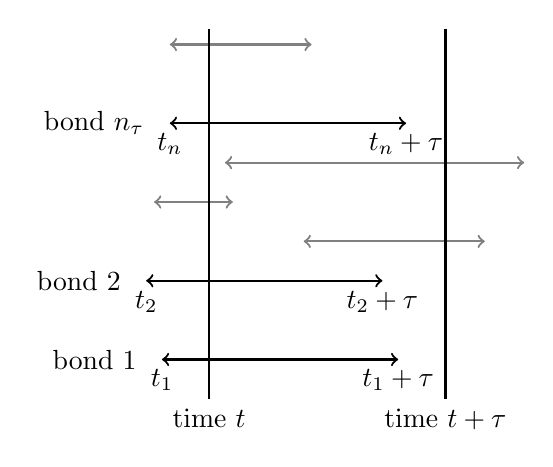
\begin{tikzpicture}[help lines/.style={thin,draw=black!50}]
%%\draw[help lines] (0,0) grid (4,4);
\draw [<->, thick] (0.4,0) node [anchor = north] {$t_1$} -- (3.4,0) node [anchor = north] {$t_1 + \tau$};
\draw (0.2,0) node [anchor = east] {bond $1$};
\draw [<->, thick] (0.2,1) node [anchor = north] {$t_2$} -- (3.2,1) node [anchor = north] {$t_2 + \tau$};
\draw (0,1) node [anchor = east] {bond $2$};
\draw [<->, thick] (0.5,3) node [anchor = north] {$t_n $} -- (3.5,3) node [anchor = north] {$t_n + \tau$};
\draw (0.3,3) node [anchor = east] {bond $n_{\tau}$};
\draw [gray,<->, thick] (1.2,2.5) -- (5.0,2.5);
\draw [gray,<->, thick] (0.3,2) -- (1.3,2);
\draw [gray,<->, thick] (2.2,1.5) -- (4.5,1.5);
\draw [gray,<->, thick] (0.5,4) -- (2.3,4) ;
\draw [thick] (1.0,4.2) -- (1.0,-0.5) node [anchor = north] {time $t$};
\draw [thick] (4.0,4.2) -- (4.0,-0.5) node [anchor = north] {time $t+\tau$};
\end{tikzpicture}
  \caption{\label{fig:P_tc} The H-bonds with lifetime $\tau$ in a certain configuration. 
At time $t$, we assume that there are totally $n_{tot}$ H-bonds can be detected, and $n_{\tau}$ H-bonds are of lifetime $\tau$, therefore,  the fraction of H-bonds that 
have the lifetime $\tau$ in the configuration at time $t$ is $P_{tc}(\tau) =  n_{\tau} /n_{tot}$.
Let $\tau$ take all the values in the interval $[0,\infty]$, we can get the HB lifetime distribution $P_{tc}(t)$.
}
\end{figure}
%\paragraph{Relation Between HB Dynamics and Anisotropy Decay}
%It is interesting to relate the HB kinetics with rotational dynamics (anisotropy decay) of single water molecules.\cite{HX01}
%
%\paragraph{Mean First Passage Time Probability Densities}

\paragraph{$k$ and $k'$: Least Squares Fit}
In order to show the effect of water molecule diffusion on the HB dynamics, we can calculate the sum of the functions $c(t)$ and $n(t)$, i.e., $c(t)+n(t)$.
%

The probability at time $t$ that a pair of water molecules bonded by H-bonds at the initial moment does not be bonded 
but the distance between their oxygen atoms is still less than $R_{OO}^c$ is 
\begin{eqnarray}
n(t) = \int_0^t dt'k_{in}(t'),
\label{eq:n_from_k_in}
\end{eqnarray}
where $k_{in}(t) = -\langle \dot h(0)[1-h(t)]h^d(t) \rangle/\langle h\rangle$ is the restricted rate function. 
Both Fig. \ref{fig:128w_bk_2delta_t_60ps_n_from_k_in}(a) and Fig.\ref{fig:128w_bk_2delta_t_60ps_n_from_k_in}(b) show the same function $n(t)$. They are calculated from 
$n(t) = \langle h(0)[1-h(t)]h^d(t) \rangle/\langle h\rangle$ and $n(t) = \int_0^t dt'k_{in}(t')$, respectively. 
In each figure, we have drawn the $n(t)$ function corresponding to the two different HB definitions. 
It can be found that neither the calculation method of $n(t)$ nor the definition of HB affects the change trend of $n(t)$, that is, 
as $t$ increases, $n(t)$ increases rapidly from 0, and it reaches a maximum value at $t \approx 10$ ps, and then gradually decreases. [EXPLAIN THE RESULTs]

%
\begin{figure}[H]
\centering
\includegraphics [width=0.6\textwidth] {./diagrams/128w_bk_2delta_t_60ps_n_from_2_methods_and_2_hb_def}
\setlength{\abovecaptionskip}{0pt}
\caption{\label{fig:128w_bk_2delta_t_60ps_n_from_k_in} 
The time dependence of the population functions $n(t)$ for bulk water, as computed from the ADH (solid line) and AHD (dashed line) 
criterion of H-bonds with the expression (a) $n(t) = \int_0^t dt'k_{in}(t')$ and (b) $n(t) = \langle h(0)[1-h(t)]h^d(t) \rangle/\langle h\rangle$, respectively.} 
\end{figure}

Khaliullin and K\"uhne have studied the H-bonding kinetics of pure water using AIMD simulations. [\cite{Khaliullin2013}]
Based on the concepts of $h(t)$, $h^{(d)}(t)$, $n(t)$ and $k(t)$, they have used the simulation data 
obtained by the AIMD simulation method to obtain the ratio $k/k'$ in the bulk water, and then the lifetime and relaxation time 
of the HB.  Here, we also use the AIMD simulation method to study the HB dynamics at the interface of LiI, NaI, and KI aqueous 
solutions. We can obtain the optimal solution range of $k$ and $k'$ from the relationship 
between the reactive flux and the HB population correlation function $c(t)$ and $n(t)$, and the parameters $k$ and $k'$, i.e.,
\begin{eqnarray}
  k(t) = kc(t)-k'n(t).
\label{eq:fitting_k_rates}
\end{eqnarray}
%
%[Answer Q3]
We can find the optimal value of the parameters, $k$ and $k'$, 
by a least squares fit of the calculated data $k(t)$, $c(t)$ and $n(t)$ beyond the transition phase.  
The functions $c(t)$, $n(t)$ and $k(t)$ can be regarded as column vectors, and denoted as ${\bf c}$, ${\bf n}$ and ${\bf k}$, respectively. 
The $k$ and $k'$ can be determined from the matrix $A = \begin{bmatrix} {\bf c} & {\bf n} \end{bmatrix}$, i.e., 
\begin{equation}
\begin{bmatrix} k\\ -k' \end{bmatrix} = (A^T A)^{-1} A^T {\bf k}. 
\end{equation}
For bulk water and the water/vapor interface, the optimal $k$ and $k'$ given by these results are reported in Table 
\ref{tab:k_k_prime_128w_pure_1} to Table \ref{tab:k_k_prime_128w_pure_5}. 
These values of the $k$ are comparable in magnitude to that obtained by Ref.\thinspace[{\cite{Khaliullin2013}}] 
% 
\begin{table}[htbp]
\centering
\caption{\label{tab:k_k_prime_128w_pure_1} 
    The $k$ and $k'$ for the bulk water and the water/vapor interface. We carried on the time region 0.2 ps $< t <$ 60 ps. 
The unit for $k$ ($k'$) is ps$^{-1}$, and that for $\tau_{\text{R}}$ ($=1/k$) is ps.} 
\begin{tabular}{ccccccc}
 Criterion & $k$  (bulk) & $k'$ (bulk) & $\tau_{\text{R}}$ (bulk) & $k$  (interf.) & $k'$ (interf.) & $\tau_{\text{R}}$ (interf.)\\
\hline
  ADH & 0.136 & 0.040 & 7.35 & 0.180 & 0.064 & 5.57  \\
  ADH(from $k_{in}$) & 0.138  & 0.058 & 7.24  & 0.184 & 0.092 & 5.43 \\
  AHD & 0.127 & 0.051 & 7.86 & 0.179  & 0.084 & 5.60\\
  AHD(from $k_{in}$) & 0.127  & 0.061 & 7.90 & 0.183  & 0.120 & 5.45 \\
\end{tabular}
\end{table}


\begin{table}[htbp]
\centering
\caption{\label{tab:k_k_prime_128w_pure_2} 
    The $k$ and $k'$ for the bulk water and the water/vapor interface. We carried on the time region 0.4 ps $< t <$ 60 ps. 
The unit for $k$ ($k'$) is ps$^{-1}$, and that for $\tau_{\text{R}}$ ($=1/k$) is ps.} 
\begin{tabular}{ccccccc}
 Criterion & $k$  (bulk) & $k'$ (bulk) & $\tau_{\text{R}}$ (bulk) & $k$  (interf.) & $k'$ (interf.) & $\tau_{\text{R}}$ (interf.)\\
\hline
  ADH & 0.127 & 0.033 & 7.87 & 0.168 & 0.055 & 5.96 \\
  ADH(from $k_{in}$) & 0.128  & 0.046 & 7.78 & 0.172  & 0.079 & 5.82\\
  AHD & 0.117 & 0.041 & 8.53  & 0.166 & 0.074 & 6.02 \\
  AHD(from $k_{in}$) & 0.117  & 0.049 & 8.57 & 0.170  & 0.104 & 5.87 \\
\end{tabular}
\end{table}


\begin{table}[htbp]
\centering
\caption{\label{tab:k_k_prime_128w_pure_3} 
    The $k$ and $k'$ for the bulk water and the water/vapor interface. We carried on the time region 0.8 ps $< t <$ 60 ps. 
The unit for $k$ ($k'$) is ps$^{-1}$, and that for $\tau_{\text{R}}$ ($=1/k$) is ps.} 
\begin{tabular}{ccccccc}
 Criterion & $k$  (bulk) & $k'$ (bulk) & $\tau_{\text{R}}$ (bulk) & $k$  (interf.) & $k'$ (interf.) & $\tau_{\text{R}}$ (interf.)\\
\hline
  ADH & 0.119 & 0.026 & 8.41 & 0.158 & 0.048 & 6.32 \\
  ADH(from $k_{in}$) & 0.120  & 0.036 & 8.35 & 0.162  & 0.069 & 6.16 \\
  AHD & 0.109 & 0.033 & 9.15 & 0.157 & 0.067 & 6.37 \\
  AHD(from $k_{in}$) & 0.108  & 0.039 & 9.20 & 0.161  & 0.093 & 6.21 \\
\end{tabular}
\end{table}

\begin{table}[htbp]
\centering
\caption{\label{tab:k_k_prime_128w_pure_4} 
    The $k$ and $k'$ for the bulk water and the water/vapor interface. We carried on the time region 1.6 ps $< t <$ 60 ps. 
The unit for $k$ ($k'$) is ps$^{-1}$, and that for $\tau_{\text{R}}$ ($=1/k$) is ps.} 
\begin{tabular}{ccccccc}
 Criterion & $k$  (bulk) & $k'$ (bulk) & $\tau_{\text{R}}$ (bulk) & $k$  (interf.) & $k'$ (interf.) & $\tau_{\text{R}}$ (interf.)\\
\hline
  ADH & 0.113 & 0.021 & 8.89  & 0.150 & 0.042 & 6.67\\
  ADH(from $k_{in}$) & 0.113  & 0.028 & 8.86  & 0.155  & 0.061 & 6.45 \\
  AHD & 0.102 & 0.026 & 9.80 & 0.149 & 0.060 & 6.69\\
  AHD(from $k_{in}$) & 0.101  & 0.031 & 9.87 & 0.154  & 0.085 & 6.48 \\
\end{tabular}
\end{table}

\begin{table}[htbp]
\centering
\caption{\label{tab:k_k_prime_128w_pure_5} 
    The $k$ and $k'$ for the bulk water and the water/vapor interface. We carried on the time region 3.2 ps $< t <$ 60 ps. 
The unit for $k$ ($k'$) is ps$^{-1}$, and that for $\tau_{\text{R}}$ ($=1/k$) is ps.} 
\begin{tabular}{ccccccc}
 Criterion & $k$  (bulk) & $k'$ (bulk) & $\tau_{\text{R}}$ (bulk) & $k$  (interf.) & $k'$ (interf.) & $\tau_{\text{R}}$ (interf.)\\
\hline
  ADH & 0.106 & 0.016 & 9.43 & 0.143 & 0.037 & 7.01\\
  ADH(from $k_{in}$) & 0.106  & 0.021 & 9.46 & 0.150  & 0.057 & 6.65\\
  AHD & 0.097 & 0.022 & 10.33 & 0.142 & 0.054 & 7.05 \\
  AHD(from $k_{in}$) & 0.096  & 0.025 & 10.43  & 0.149  & 0.080 & 6.70 \\
\end{tabular}
\end{table}

For the water/vapor interface, we also calculated the constants $k$ and $k'$ by least square fit. 

\begin{figure}[H]
\centering
\includegraphics [width=0.6\textwidth] {./diagrams/128w_itp_50ps_n_from_2_methods_and_2_hb_def}
\setlength{\abovecaptionskip}{0pt}
\caption{\label{fig:128w_itp_50ps_n_from_2_methods_and_2_hb_def} 
The time dependence of the population functions $n(t)$ for water/vapor interface, as computed from the ADH (solid line) and AHD (dashed line) 
criterion of H-bonds with the expression (a) $n(t) = \int_0^t dt'k_{in}(t')$ and (b) $n(t) = \langle h(0)[1-h(t)]h^d(t) \rangle/\langle h\rangle$, respectively.} 
\end{figure}

\newpage
\section{Water-water Pair Based Hydrogen Bond Dynamics}
The method described in this paragraph is used more in the literature. 
The basis is the population operator $h(t)$ of the HB formed between two water molecules. 
We use the correlation function \CHB to describe the relaxation of H-bonds between two water molecules: [\cite{Luzar1994,AL96,AC00}]
\begin{eqnarray}
C_{\text{HB}}(t)=\langle h(0)h(t) \rangle/\langle h\rangle
\label{eq:C_HB}.
\end{eqnarray}
Similarly, with the aid of the ergodic principle, the ensemble average $\langle \cdots\rangle$ is implemented by time average.
The $\langle h\rangle$ is the probability that a pair of randomly chosen water molecules in the system is
H-bonded at any time $t$. 

The function \CHB is interpreted as the probability that the HB between a certain pair of water molecules is intact at time  $t$, 
if the pair of water molecules are H-bonded at time zero. 
In a large system that consist of many water molecules, the probability that a specific pair of water molecules are H-bonded is extremely small. 
Therefore, the \CHB relaxes to zero, when $t$ is large enough. 
The \CHB measures correlation in $h(t)$ independent of any possible bond breaking events. 
It is one of the intermittent HB correlation functions, introduced by Rapaport, [\cite{DCR83}] 
and can be studied by a continuous function, probability densities.
From the \CHB, the HB relaxation time is computed as [\cite{Lee2007}]


Fig.\ref{fig:128w_bk_2delta_t_60ps_water_pair_c_ns40} shows the correlation function $C_{HB}(t)$ defined by $C_{HB}(t) = \langle h(0)h(t)\rangle/\langle h \rangle$ for bulk water over time. The result is calculated by DFTMD simulation, and the temperature is 300 K. 
\begin{figure}[H]
\centering
\includegraphics [width=0.5\textwidth] {./diagrams/128w_bk_2delta_t_60ps_water_pair_c_ns40}
\setlength{\abovecaptionskip}{0pt}
\caption{\label{fig:128w_bk_2delta_t_60ps_water_pair_c_ns40} 
The correlation functions $C_{HB}(t)$ for bulk water, based on water-water pair hydrogen bond population operator $h(t)$, as computed from the ADH (solid line) and AHD (dashed line) criterion of H-bonds. [DESCRIBE THE FIGURE][COMPARE THE RESULTs TO hbond-based CORRELATION FUNCTION]} 
\end{figure}


\section{Rotational Anisotropy Decay of Water at the Interface of Alkali-Iodine Solutions}\label{CHAPETR_AD}
Using the transition dipole auto-correlation function, 
we determined the rotational anisotropy decay and therefore the OH-stretch relaxation at water/vapor interface of alkali iodide solutions.
%The effects of ion environment on structure and dynamics of water are obtained by comparing the second-order Legendre polynomial, i.e.,  $P_2(x)=\frac{1}{2}(3x^2-1)$,  orientational correlation function of the transition dipole.
The anisotropy decay can be determined from experimental signal in two different polarization configurations---parallel and perpendicular polarizations, by 
\begin{equation}
        R(t)=\frac{S_{\parallel}(t)-S_{\perp}(t)}{S_{\parallel}(t)+2S_{\perp}(t)}
\label{eq:ad}
\end{equation}
where $t$ is the time between pump and probe laser pulses.  The anisotropy decay can also be obtained by simulations, and calculated by the third-order response functions $R(t)$. [\cite{Jansen10,Jansen06}]
%
%In the first shell with a radius 3 \A, the entropy difference betweem the \Li shell and \Na shell,
%$\Delta S=k_B\text{ln}\frac{\Omega_\text{Na}}{\Omega_\text{Li}}=k_B\text{ln}\frac{n_\text{Na}/V_\text{Na}}{n_\text{Li}/V_\text{Li}} =k_B\text{ln}1.05$.
%
%\paragraph{Probability Distribution of Ions}
%The probability distribution, shown in Fig.~\ref{fig: prob_124_LiI_Sans_double_axis}, of the ions in the water/vapor interface of LiI and NaI solutions with repect to the depth of the ions in the solutions 
%indicates that the \I ions prefer to staying at the topmost layer of surface of solutions.
%(molar concentration: 0.9 M, temperature: 330 K) 
%It shows that \I ions tend to the surface of the solutions, while \Na and \Li tend to stay in the bulk. This result is consistent with the calculations from Ishiyama and Morita\cite{TI07,TI14}.
The orientational anisotropy $C_2(t)$ is given by the rotational time-correlation function 
\begin{equation}
C_2(t)=\langle P_2(\hat{u}(0)\cdot\hat{u}(t)) \rangle,
\label{eq:tcf2}
\end{equation}
where $\hat{u}(t)$ is the time dependent unit vector of the transition dipole, $P_2(x)$ is the second Legendre polynomial, and $\langle \rangle$ indicate 
equilibrium ensemble average. [\cite{Corcelli05,LinYS2010}] %\cite{2010Lin} % angular brackets

The anisotropy decay $C_2(t)$ for the water/vapor interface of LiI solution is shown in Fig.\space\ref{fig:c2_2LiI_16_inset}.
This function decays faster than that of neat water, indicating that H-bonds
at the interfaces of alkali-iodine solutions reorient faster than in neat water. The inset shows the first 0.4 ps of $C_2(t)$, from which we see a 
quick change during the first $\sim 0.1$ ps primarily due to librations.
%
\begin{figure}[h]
\centering
\includegraphics [width=0.6\textwidth] {./diagrams/c2_2LiI_16_inset} 
\setlength{\abovecaptionskip}{0pt}
  \caption{\label{fig:c2_2LiI_16_inset} The time dependence of the $C_2(t)$ of OH bonds at the water/vapor interfaces of 0.9 M LiI solution and of neat water (dashed line) at 330 K, calculated by DFTMD simulations. The water/vapor interface of neat water is modeled with a slab made of 121 water molecules in a simulation box of size $15.6 \times 15.6 \times 31.0$ \A$^3$.}
\end{figure}
%
We also calculated the $C_2(t)$ for the interface of other alkali-iodine solutions LiI and KI. 
The results of $C_2(t)$ for the water/vapor interfaces of these solutions are shown in Fig.\space\ref{fig:c2_2KI_2NaI_2LiI_16}.
In all the cases $C_2(t)$ decays faster than in neat water, indicating that H-bonds
at the interfaces of the three alkali-iodine solutions are orientated faster than that of neat water.
They show that \I ions can accelerate the dynamics of molecular reorientation of water molecules at interfaces.   

%
\begin{figure}[htbp]
\centering
\includegraphics [width=0.6 \textwidth] {./diagrams/c2_2KI_2NaI_2LiI_16} 
\setlength{\abovecaptionskip}{0pt}
  \caption{\label{fig:c2_2KI_2NaI_2LiI_16} The time dependence of the $C_2(t)$ of OH bonds in water molecules at the water/vapor 
  interface of 0.9 M alkali-iodine solutions and of neat water (dashed line) at 330 K, calculated by DFTMD simulations.}
\end{figure} 

We have obtained non-single-exponential kinetics for the rotation of water molecules both at the surface 
and in bulk water (Appendix \ref{single_exp}).
%This result is true for water molecules bound to ions. 
Therefore, the rotational motion of water molecules are not simply characterized by well-defined rate constants. 
%Then the problem is to understand the kinetics.
Similar non-single-exponential kinetics is also obtained in the HB kinetics
in liquid water [\cite{AL96,Dirama05}] and in the time variation of the average frequency shifts of the 
remaining modes after excitation in hole burning technique [\cite{Rey2002,Moller2004}] and using BLYP functional. [\cite{Bankura2014}]
Luzar and Chandler interpreted 
the non-single-exponential kinetics as the result of an interplay between 
diffusion and HB dynamics. [\cite{AL96}] 
We can understand the non-single-exponential kinetics of rotational 
anisotropy decay by fitting the rotational anisotropy decay by a 
biexponential function.

To obtain the effects of diffusion and HB decay of water molecules
in solutions respectively, we assume that there are two independent 
decays in the process of an anisotropy decay. 
Therefore, the $C_2(t)$ has the form [\cite{TanHS05}]
\begin{equation}
C_2(t)=A_1e^{-\kappa_1 t} +A_2e^{-\kappa_2 t},
\label{eq:tcf3}
\end{equation}
where $A_i$ are constants and $\kappa_i$ are decay rates ($i=1, 2$). 
The time constants and amplitudes of the biexponentials fits for 
the $C_2(t)$ are listed in Table ~\ref{tab:2LiI_c2_biexp} and Table ~\ref{tab:2NaI_c2_biexp}.
The biexponential fit is very close to the calculated $C_2(t)$, which can be seen in Fig.\space\ref{fig:2LiI-124w_c2_fit_5ps_biexp} (compare Fig.\space\ref{fig:2LiI-124w_c2_fit_5_single-exp}).
%
\begin{table}[hbt]
\centering
\caption{\label{tab:2LiI_c2_biexp}%
	Biexponential fitting (5 ps) of the $C_2(t)$ for water molecules in 0.9 M LiI solution.}
%\begin{ruledtabular}
\begin{tabular}{lccccc}
water molecules & $A_1$  & $\kappa_1$ (THz) & $A_2$ & $\kappa_2$ (THz) \\
\hline
I$^-$-shell & 0.44 & 0.25 & 0.39 & 0.26\\
Li$^+$-shell & 0.88 & 0.07 & 0.07 & 8.24\\
bulk & 0.84 & 0.11 & 0.09 & 4.88 \\
surface & 0.73 & 0.27 & 0.22 & 13.47 \\
\end{tabular}
%\end{ruledtabular}
\end{table}
%--

\begin{table}
\centering
  \caption{\label{tab:2NaI_c2_biexp}%
	Biexponential fitting (5 ps) of the $C_2(t)$ for water molecules in 0.9 M NaI solution.}
  \begin{tabular}{lccccc}
  water molecules & $A_1$  & $\kappa_1$ (THz) & $A_2$ & $\kappa_2$ (THz) \\
  \hline
  I$^-$-shell & 0.86 & 0.14 & 0.08 &9.86 \\
  Na$^+$-shell & 0.71 & 0.06 & 0.18 &0.79 \\
  bulk & 0.81 & 0.06 & 0.10 & 1.25 \\
  surface & 0.77 & 0.11 & 0.13 & 2.31 \\
  \end{tabular}
\end{table}
%
%图
\begin{figure}[htbp]
\centering
\includegraphics [width= \textwidth] {./diagrams/2LiI-124w_c2_fit_5_biexp} 
  \caption{\label{fig:2LiI-124w_c2_fit_5ps_biexp} The time dependence of the $C_2(t)$ of OH bonds 
  in water molecules at the water/vapor interface of LiI solution.}
\end{figure} 
%
%[Notes: The 63-water-slab models is listed here as a reference. The number of water molecules is small; The data for KI/vapor and LiI/vapor interfaces come from  KI\_16 and LiI\_16 systems.  
%Water(63) &0.831$\pm(1\times10^{-4})$ &  0.08760 $\pm(2\times 10^{-5})$&0.100$\pm(2\times10^{-4})$ & 1.029 $\pm(4\times10^{-3})$  \\ ]
%
%\begin{figure}[htbp]
%\centering
%\includegraphics [width=0.4 \textwidth] {./diagrams/c2_121-pure_2KI_2LiI_16_inset_fit_biexp} 
%\setlength{\abovecaptionskip}{10pt}
%\caption{\label{fig:c2_121-pure_2KI_2LiI_16_inset_fit_biexp} The fitted and calculated anisotropy decay of OH bonds in water molecules in LiI solution/vapor interface (red), LiI solution/vapor interface (blue) and neat water/vapor interface (black). The corresponding fitted functions are denoted by dashed lines. The concentration of LiI and KI solution is 0.9 M.}
%\end{figure} 

Then we considered the effect of ion species in solutions on the anisotropy decay of water molecules.
From Table \ref{tab:2LiI_c2_biexp} and Table \ref{tab:2NaI_c2_biexp}, we find that 
for both LiI and NaI solutions, there are two decay processes in the dynamics --- amplitude $\sim 1$,
decay constant $\sim$ 0.1 THz, and for the other describe the initial fast decay 
of the anisotropy, with amplitude $\sim 0.1$, decay constant $\sim$ (1--10) THz, 
due to the inertial-librational motion preceding the orientational diffusion.
That is, two decay processes exist in the dynamics of water molecules 
at the water/vapor interfaces of alkali-iodine solutions. 
%The one describe the initial fast decay of the anisotropy, 
%with amplitude $\sim$ 0.1, decay constant $\sim$ (1--10) THz,
%results from the inertial-librational motion preceding the orientational diffusion.
%
\begin{table}[H]
\centering
\caption{\label{tab:fitting_c2_for_each_type_of_water}%
  Biexponentially fitting (2 ps) of the $C_2(t)$ for different types of water molecules at the water/vapor interface of LiI solutions.}
\begin{tabular}{lccccc}
water molecules & $A_1$  & $\kappa_1$ (THz) & $A_2$ & $\kappa_2$ (THz) \\
\hline
$DDAA$ & 0.85 & 0.25   & 0.10 & 16.0\\
$DD'AA$ & 0.89 & 0.14  & 0.06 & 14.1 \\
$D'AA$ & 0.38 & 0.99 & 0.38 & 0.99 \\
\end{tabular}
\end{table}
%
\begin{table}[H] %[!hbtp]
\centering
\caption{\label{tab:table_CoordNo}%
The coordination number of the atoms in LiI (NaI) solutions.}
\begin{tabular}{lccc}
name & radius of the first shell (\AA) & coordination number \\
\hline
$n_\text{I-H}(\text{LiI})$ & 3.3 & 5.5 \\
$n_\text{I-H}(\text{NaI)}$ & 3.3 & 5.1 \\
$n_\text{I-O}(\text{LiI)}$ & 4.3 & 5.8 \\
$n_\text{I-O}(\text{NaI)}$ & 4.3 & 6.0 \\
$n_\text{Li-O}(\text{LiI)}$ & 3.0 & 4.0 \\
$n_\text{Na-O}(\text{NaI)}$ & 3.5 & 6.0 
\end{tabular}
\end{table}

\section{I$^-$--Water Hydrogen Bonds in Aqueous Solutions}
In the case of water--water hydrogen bonds, the critical distance of $R_c^{OO}=3.5$ \AA are the position of the first minimum of the oxygen--oxygen RDF.
For the anion--oxygen hydrogen bonds, we can use the similar criteria. The cutoff values for $X$--oxygen distance are obtained from the positions of the first
minimum of the $X$--oxygen RDF, i.e., $R_c^{XO}=4.1$, 3.7 \A, for $X$ = I$^-$ and nitrate O. We have still used $30^{\circ}$ for the anglar cutoff.\cite{Chowdhuri2006}
\begin{figure}[htbp]
\centering
\includegraphics [width=0.6 \textwidth] {./diagrams/gdr_127_LiNO3} 
\setlength{\abovecaptionskip}{0pt}
  \caption{\label{fig:gdr_127_LiNO3} (a)Li--water O, Li--water H RDFs; (b) Nitrate O--water O, nitrate O-water H RDFs for LiNO$_3$ solutions at 300 K. The RDFs were computed from DFTMD.}
\end{figure}
The function $C_{HB}$ of I$^-$--water and water--water hydrogen bonds describes the structural relaxation of these H- bonds. The results of the $C_{HB}(t)$ are shown in Figure \ref{fig:X-O_c_lii}. 
\begin{figure}[htbp]
\centering
\includegraphics [width=0.6 \textwidth] {./diagrams/X-O_c_lii} 
\setlength{\abovecaptionskip}{0pt}
  \caption{\label{fig:X-O_c_lii} Time dependence of the intermittent correlation functions of I$^-$--water (I$^-$--W) and water--water hydrogen bonds at 300 K.}
\end{figure}
The results of the continuous correlation functions for both definitions (ADH and AHD criterions) for the H-bonds are shown in Figure \ref{fig:wat-wat_s_lii} 
for I$^-$--water hydrogen bonds. The results of water--water hydrogen bonds are also included for comparison in both Figure \ref{fig:wat-wat_s_lii} (a) and (b).
\begin{figure}[htbp]
\centering
\includegraphics [width=0.6 \textwidth] {./diagrams/wat-wat_s_lii} 
\setlength{\abovecaptionskip}{0pt}
  \caption{\label{fig:wat-wat_s_lii} Time dependence of the continuous correlation functions of I$^-$--water (I$^-$--W) and water--water hydrogen bonds at 300 K.}
\end{figure}
For both definitions for the H-bonds, it is found that the I$^-$--water hydrogen bonds show faster dynamics than water--water hydrogen bonds. 
(consistent to the previous MD results.) Therefore, the time scales of the relaxation of these H-bonds can be obtained for both definitions. 
In Table \ref{tab:properties_anion-water_hbs}, we have included the average lifetimes $\langle\tau_{a}\rangle$, which can be cumputed from Eq.\ref{eq:calculate_hb_lifetime}, 
for both water--water and I$^-$--water hydrogen bonds. We performing the fitting in the time region 0.2 ps < $t$ < 12 ps to calculate the forward and backward rate constants
for HB breaking.
%
\begin{table}[htbp]
\centering
\caption{ 
    The Dynamical properties of anion--water and water--water hydrogen bonds at 300 K. Data are from DFTMD for the aqueous solutions. The values are expressed in ps.} 
\begin{tabular}{ccccc}
\label{tab:properties_anion-water_hbs}
 Quantity & Criterion & W--W & I$^-$--W & NO$_3^-$--W  \\
\hline
  $\langle\tau_a\rangle$  & ADH & 190.3 & 0.10 & 4.35 \\
  $\langle\tau_a\rangle$ & AHD & 186.8  & 0.11 & 7.91 \\
  $1/k$ & ADH & 9.82 & 2.80 & 4.15 \\
  $1/k$ & AHD & 8.97 & 2.40 & 6.02\\
\end{tabular}
%
% Data from: LiI solution:  gang@XPS /home/gang/Github/water_pair_HB_dynamics/src/least_square_fit
% Data from: LiNO3 solution:  /home/gang/Github/water_pair_HB_dynamics/src/least_square_fit/LiNO3 
\end{table}
\begin{figure}[htbp]
\centering
\includegraphics [width=0.6 \textwidth] {./diagrams/I--wat_n_lii} 
\setlength{\abovecaptionskip}{0pt}
  \caption{\label{fig:I--wat_n_lii} Time dependence of the correlation functions $n_{HB}(t)$ of I$^-$--water (I$^-$--W) and water--water hydrogen bonds at 300 K.}
\end{figure}

